\documentclass[10pt, a5paper]{article}
\usepackage{pdfpages}
\usepackage{parallel}
\usepackage[T2A]{fontenc}
\usepackage{ucs}
\usepackage[utf8x]{inputenc}
\usepackage[polish,english,russian]{babel}
\usepackage{hyperref}
\usepackage{rotating}
\usepackage[inner=2cm,top=1.8cm,outer=2cm,bottom=2.3cm,nohead]{geometry}
\usepackage{listings}
\usepackage{graphicx}
\usepackage{wrapfig}
\usepackage{longtable}
\usepackage{indentfirst}
\usepackage{array}
\newcolumntype{P}[1]{>{\raggedright\arraybackslash}p{#1}}
\frenchspacing
\usepackage{fixltx2e} %text sub- and superscripts
\usepackage{icomma} % коскі ў матэматычным рэжыме
\PreloadUnicodePage{4}

\newcommand{\longpage}{\enlargethispage{\baselineskip}}
\newcommand{\shortpage}{\enlargethispage{-\baselineskip}}

\def\switchlang#1{\expandafter\csname switchlang#1\endcsname}
\def\switchlangbe{
\let\saverefname=\refname%
\def\refname{Літаратура}%
\def\figurename{Іл.}%
}
\def\switchlangen{
\let\saverefname=\refname%
\def\refname{References}%
\def\figurename{Fig.}%
}
\def\switchlangru{
\let\saverefname=\refname%
\let\savefigurename=\figurename%
\def\refname{Литература}%
\def\figurename{Рис.}%
}

\hyphenation{admi-ni-stra-tive}
\hyphenation{ex-pe-ri-ence}
\hyphenation{fle-xi-bi-li-ty}
\hyphenation{Py-thon}
\hyphenation{ma-the-ma-ti-cal}
\hyphenation{re-ported}
\hyphenation{imp-le-menta-tions}
\hyphenation{pro-vides}
\hyphenation{en-gi-neering}
\hyphenation{com-pa-ti-bi-li-ty}
\hyphenation{im-pos-sible}
\hyphenation{desk-top}
\hyphenation{elec-tro-nic}
\hyphenation{com-pa-ny}
\hyphenation{de-ve-lop-ment}
\hyphenation{de-ve-loping}
\hyphenation{de-ve-lop}
\hyphenation{da-ta-ba-se}
\hyphenation{plat-forms}
\hyphenation{or-ga-ni-za-tion}
\hyphenation{pro-gramming}
\hyphenation{in-stru-ments}
\hyphenation{Li-nux}
\hyphenation{sour-ce}
\hyphenation{en-vi-ron-ment}
\hyphenation{Te-le-pathy}
\hyphenation{Li-nux-ov-ka}
\hyphenation{Open-BSD}
\hyphenation{Free-BSD}
\hyphenation{men-ti-on-ed}
\hyphenation{app-li-ca-tion}

\def\progref!#1!{\texttt{#1}}
\renewcommand{\arraystretch}{2} %Іначай формулы ў матрыцы зліпаюцца з лініямі
\usepackage{array}

\def\interview #1 (#2), #3, #4, #5\par{

\section[#1, #3, #4]{#1 -- #3, #4}
\def\qname{LVEE}
\def\aname{#1}
\def\q ##1\par{{\noindent \bf \qname: ##1 }\par}
\def\a{{\noindent \bf \aname: } \def\qname{L}\def\aname{#2}}
}

\def\interview* #1 (#2), #3, #4, #5\par{

\section*{#1\\{\small\rm #3, #4. #5}}

\def\qname{LVEE}
\def\aname{#1}
\def\q ##1\par{{\noindent \bf \qname: ##1 }\par}
\def\a{{\noindent \bf \aname: } \def\qname{L}\def\aname{#2}}
}

\begin{document}
\title{codename: Taurus}
\author{Taras Svirinovski, Minsk, Belarus}
\maketitle
\begin{abstract}
Taurus is automation-friendly framework for Load Testing.
\end{abstract}
В статье рассматривается инструмент для простого доступа к различным средствам автоматизированного нагрузочного тестирования WEB-ресурсов.

\subsection*{Введение в нагрузочное тестирование}

Нередко можно встретить снисходительное отношение к тестированию со стороны программистов, поэтому мы позволим себе объяснить важность предметной области и заодно провести маленький ликбез.

Вообразите себя владельцем интернет-магазина. Через месяц грядут большие распродажи и вы не знаете "--- ожидает вас рост объёмов или падение сервера и язвительные шутки конкурентов (впрочем, если вы известный монополист авиаперевозок "--- дальше можете не читать). Вот если бы эти пользователи набежали прямо сейчас, то, оценив нагрузку, вы бы добавили нужных ресурсов. Но каких именно? Памяти или процессоров? Или дискового кэша? А может всё и так хорошо?
Определенность в данной ситуации "--- большое конкурентное преимущество для бизнеса и он ставит задачу: создать виртуальную нагрузку. Пусть два бота кладут товары в корзину, один пытается оплатить ещё один отменяет заказ и три в это время регистрируются, итого "--- семь. Или семь миллионов "--- как пожелает тот, кто создает нагрузку.

Здесь пора обозначить два понятия: \emph{генератор нагрузки} (приложение, возможно много копий одного приложения в облаке, эмулирующие пользователей) и \emph{тест-план} "--- сценарий поведения бота.

\subsection*{Существующие инструменты}

Люди, имеющие отношение к обсуждаемой области, обязательно слышали про JMeter, Gatling, Selenium, более опытные могут упомянуть ещё с полдюжины средств генерации нагрузки. Итак, первая проблема "--- этих средств просто много и они совершенно разные. ctoНекоторые, как JMeter, для описания тест-плана требуют использования графического интерфейса, другие, как Gatling, опираются внутри на классические языки программирования (Scala, Java, Python). У них отличаются умолчания, способности распределенного выполнения и даже наличие такого базового функционала, как возможность поддерживать нагрузку определенное время. Эти инструменты имеют разную способность к автоматизации "--- некоторые, о ужас, возвращают успешный код завершения когда тест провалился. Люди, отвечающие за работу CI, понимают, что проверять систему подобными инструментами становится крайне неудобно. Впрочем, есть одна область, в которой традиционные инструменты нагрузочного тестирования достаточно близки: результаты их работы сложно увидеть, а увидев "--- почти невозможно понять.

\subsection*{Наш подход}

Я прошу прощения если вы эксперт в данной области и описанные сложности кажутся вам надуманными. Вы, не просыпаясь, в уме разбираете километровые csv-файлы с timestamp’ами в UTC и ваш мощный скрипт рисует рисует графики, от которых в восхищении весь совет директоров. У меня для вас плохие новости: мы решили снизить планку входа в нагрузочное тестирование. Это не обязательно означает помочь вчерашним студентам начать карьеру в IT "--- нередко в нагрузочное тестирование приходят и опытные разработчики, с одной стороны, предпочитающие аскетичный внешний вид и ясные конфигурационные файлы а с другой, "--- активно использующие автоматизацию и нуждающиеся в свежих наработках индустрии. Мы в BlazeMeter проанализировали существующие инструменты и решили, что знаем, как упростить жизнь и новичкам, и экспертам.

Чтобы попробовать Taurus, нам понадобится:

\begin{enumerate}
  \item установить инструмент (проще всего "--- из репозитория пакетов Python утилитой pip, но есть и нативные установщики для различных OS и даже образ для Docker’a)
  \item создать конфигурационный файл для описания тест-плана:
\lstset{ %
anguage=C,                 % выбор языка для подсветки (здесь это С)
basicstyle=\small\sffamily, % размер и начертание шрифта для подсветки кода
breaklines=true,           % автоматически переносить строки (да\нет)
breakatwhitespace=false, % переносить строки только если есть пробел
}

\begin{lstlisting}

execution:
- concurrency: 100
  ramp-up: 1m
  hold-for: 5m
  scenario: quick-test
scenarios:
  quick-test:
    requests:
\end{lstlisting}
\end{enumerate}

\begin{enumerate}
  \item запустить инструмент, передав ему параметром конфигурационный файл
	\verb@$ bzt <test_file>@
\end{enumerate}

Открывающийся после этого при настройках по умолчанию псевдографический мониторинг не только вызывает вау-эффект у настоящих гиков, но и неплохо позволяет анализировать тест в динамике:

\begin{figure}[h!]
  \centering
  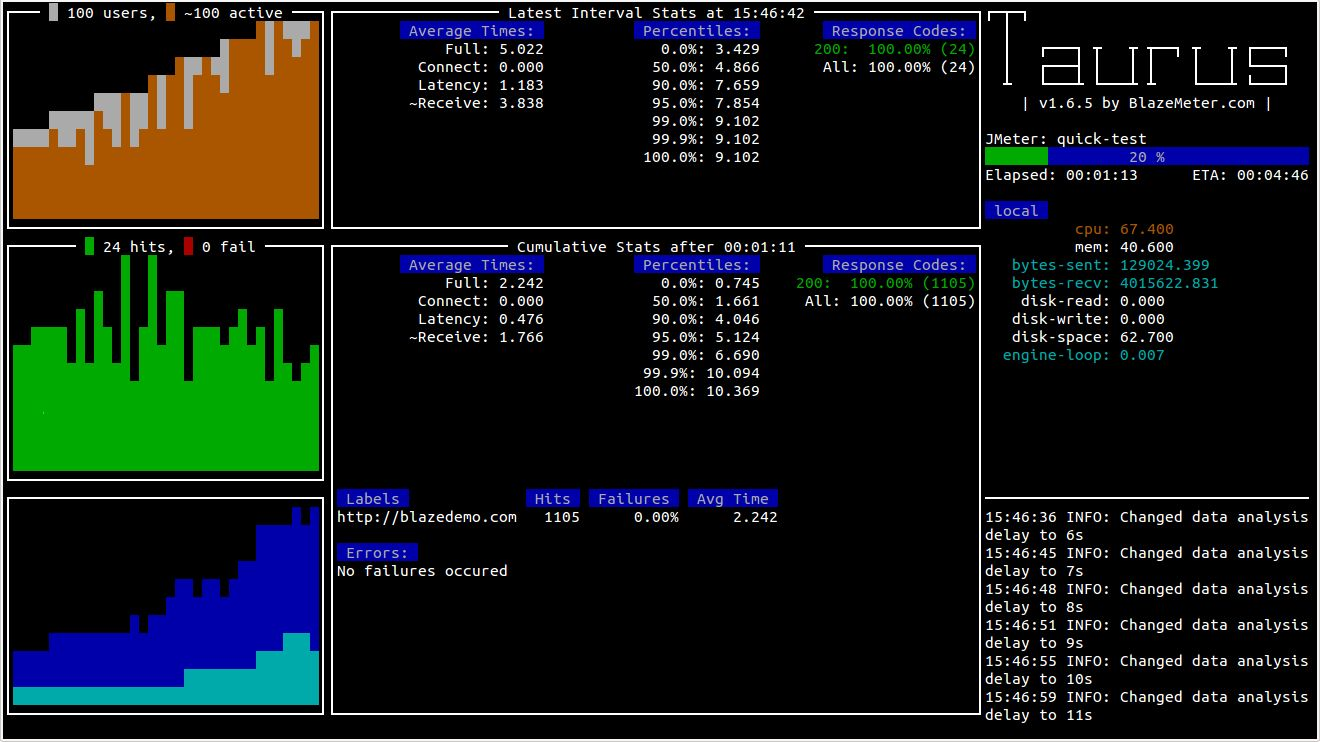
\includegraphics[height=4.5cm]{15_2016_Svirinovski1.png}
\end{figure}

\subsection*{Как это готовить правильно?}

Конфигурационный файл может быть написан на YAML либо JSON. На вышеприведенном примере рассмотрим синтаксис первого из них. Файл должен начинаться с трех дефисов, отступы задают иерархию, основные строительные элементы "--- списки и словари, один элемент структуры на строку. Этих знаний достаточно, чтобы понимать и модифицировать образцы (например, с сайта gettaurus.org).

Приложение консольное, вопросов не задает и сходу встраивается в любую автоматизацию. На это хотелось бы обратить особое внимание: не просто совместимость, но удобство применения, скажем, для Continuous Integration "--- едва ли не основной принцип проекта. Добавлением нескольких строчек возможно:

\begin{itemize}
  \item запустить одновременно несколько генераторов нагрузки;
  \item отложить тест на определенное время;
  \item настроить критерии успешности теста в том числе и на основании полученных http-пакетов;
  \item менять исполнителя "--- например, потребление ресурсов \linebreak JMeter’ом вас не устраивает или нужны возможности \linebreak Selenium’а;
  \item использовать разные типы http-запросов, добавлять заголовки и т.д.;
  \item получить web-отчет, ссылку на который можно отправить коллеге;
  \item перенести тест в облако и выполнить на десятках виртуальных машин (осторожно, это может быть платно, о чем я расскажу ниже).
\end{itemize}

Сейчас мы поддерживаем девять генераторов нагрузки "--- JMeter, Selenium, Gatling, Grinder, Locust, PBench, Siege, Apache Benchmark и Tsung.

Taurus преобразовывает конфигурационные параметры в опции, понятные конкретному генератору. Для JMeter генерируется XML (JMX), для Gatling "--- код на Scala (разумеется, выполнение уже готовых нативных тестовых скриптов также возможно). При необходимости Taurus скачивает инструмент из сети, запускает, следит за работой показывая промежуточные результаты (более или менее в реальном времени) и в конце теста выдает финальный отчет.

Отдельно нужно коснуться некоторых принципов выдачи результатов. 
Данные агрегируются по временным интервалам и выделяются настраиваемыми перцентилями "--- так, например, инженеру будет интересно, уложились ли 98\% запросов в лимит времени. При этом результаты различных инструментов выглядят одинаково и могут сравниваться по основным метрикам.

Ещё пользователь может:

\begin{itemize}
  \item выполнять мониторинг ресурсов как генерующей нагрузку системы, так и нагружаемой "--- очевидно, истощение ресурсов любой из них тестировщику следует знать;
  \item производить быструю настройку переопределяя элементы конфигурации из командной строки;
  \item структурировать тест-план используя включаемые файлы;
  \item определять команды операционной системы для выполнения на разных этапах теста.
\end{itemize}

Для специалистов замечу, что основным поддерживаемым инструментом является JMeter, так уж сложился спрос в индустрии.

\subsection*{Работа изнутри, перспективы}

В данный момент разработка идет силами трех человек программистов. Исходный код публично на Github, поддержка пользователей идет посредством Google Groups. Для контроля качества кода изменения оформляются pullrequest’ами, проходящими обязательное review. Выделенных тестировщиков нету, их роль играет армия пользователей, на сообщения которых мы стараемся реагировать \textbf{безотлагательно}. 
Код основательно покрыт юнит-тестами (на данный момент покрытие составляет 92\%).

Сборку и деплой пакета и сайта Taurus’a осуществляет Jenkins, выполняя перед этим функциональное и unit-тестирование. Для проверки commit’ов используются также Travis и Appveyor. JIR’ы у нас нету, и github’овский issue tracker отключен по вышеупомянутым соображениям "--- основная идея поддержки заключается в том, чтобы исправлять выявленные баги немедленно.

Можно уверенно говорить что мы уже стали полезны "--- в этом году нас почтил вниманием devops.com. Развитие идет достаточно активно, по крайней мере, новый функционал добавляется в планы быстрее, чем реализовывается.

BlazeMeter достаточно ненавязчиво продвигает некоторую интеграцию со своим сервисом "--- как я уже говорил, web-отчеты на их сайте, одна виртуальная машина бесплатно для облачного исполнения, некоторые сложные конвертации форматов.

Основная задача, которую ставит перед нами BlazeMeter "--- делать удобный продукт, который привлечет ощутимую часть сообщества, поэтому многие новые направления вырастают из хотелок пользователей. Из подобных глобальных вещей могу отметить скорый приход поддержки функционального тестирования, валидацию конфигурационных файлов, скоростную фотосъемку загрузки web-страницы, поддержку Selenium-тестов на .Net и JS.

\subsection*{Как мы дошли до такой жизни}

Компания BlazeMeter, зарегистрированная в США и имеющая команду разработки в Израиле, уже около пяти лет предлагает средства для тестирования формата <<поставь галочки на сайте, а мы за тебя создадим нагрузку и покажем отчёт>>.

В поисках новых ниш компания обратила внимание на инженеров. Даже не принося деньги напрямую довольные технически грамотные люди создают очень полезный с точки зрения IT-бизнеса фон, недостижимый, например, рекламой или скидками. Этим клиентам не лень читать документацию, но им нужны очень мощные и гибкие инструменты, а ещё лучше "--- поддержка тех инструментов, которые они уже используют (много ли среди нас желающих переучиваться?). А то, что они используют, оставляет желать лучшего "--- значит, есть где приложить силы и получить хорошую репутацию.

Языком для проекта был выбран Python, отлично подходящий для работы со сторонними инструментами в командной строке на различных архитектурах, лицензией "--- Apache 2.0. Архитектура модульная, многие компоненты вполне могут быть переписаны программистом средней руки (поддержка новых генераторов нагрузки или специфический репортер, скажем, отправляющий \linebreak SMS-сообщения).

Так работает Taurus "--- швейцарский нож для инструментов нагрузочного тестирования, дающий пользователям удобный интерфейс взаимодействия с ними (стараясь при этом не потерять некоторые изюминки отдельных генераторов).

\end{document}
